\section{态的迭加}

\begin{quotation}
``创造的源泉在于数学,因此,从某个意义上讲,我认为,纯思维可以掌握现实,像古人所梦想的那样。''\qquad 爱因斯坦
\end{quotation}


\begin{figure}[h]
\begin{center}
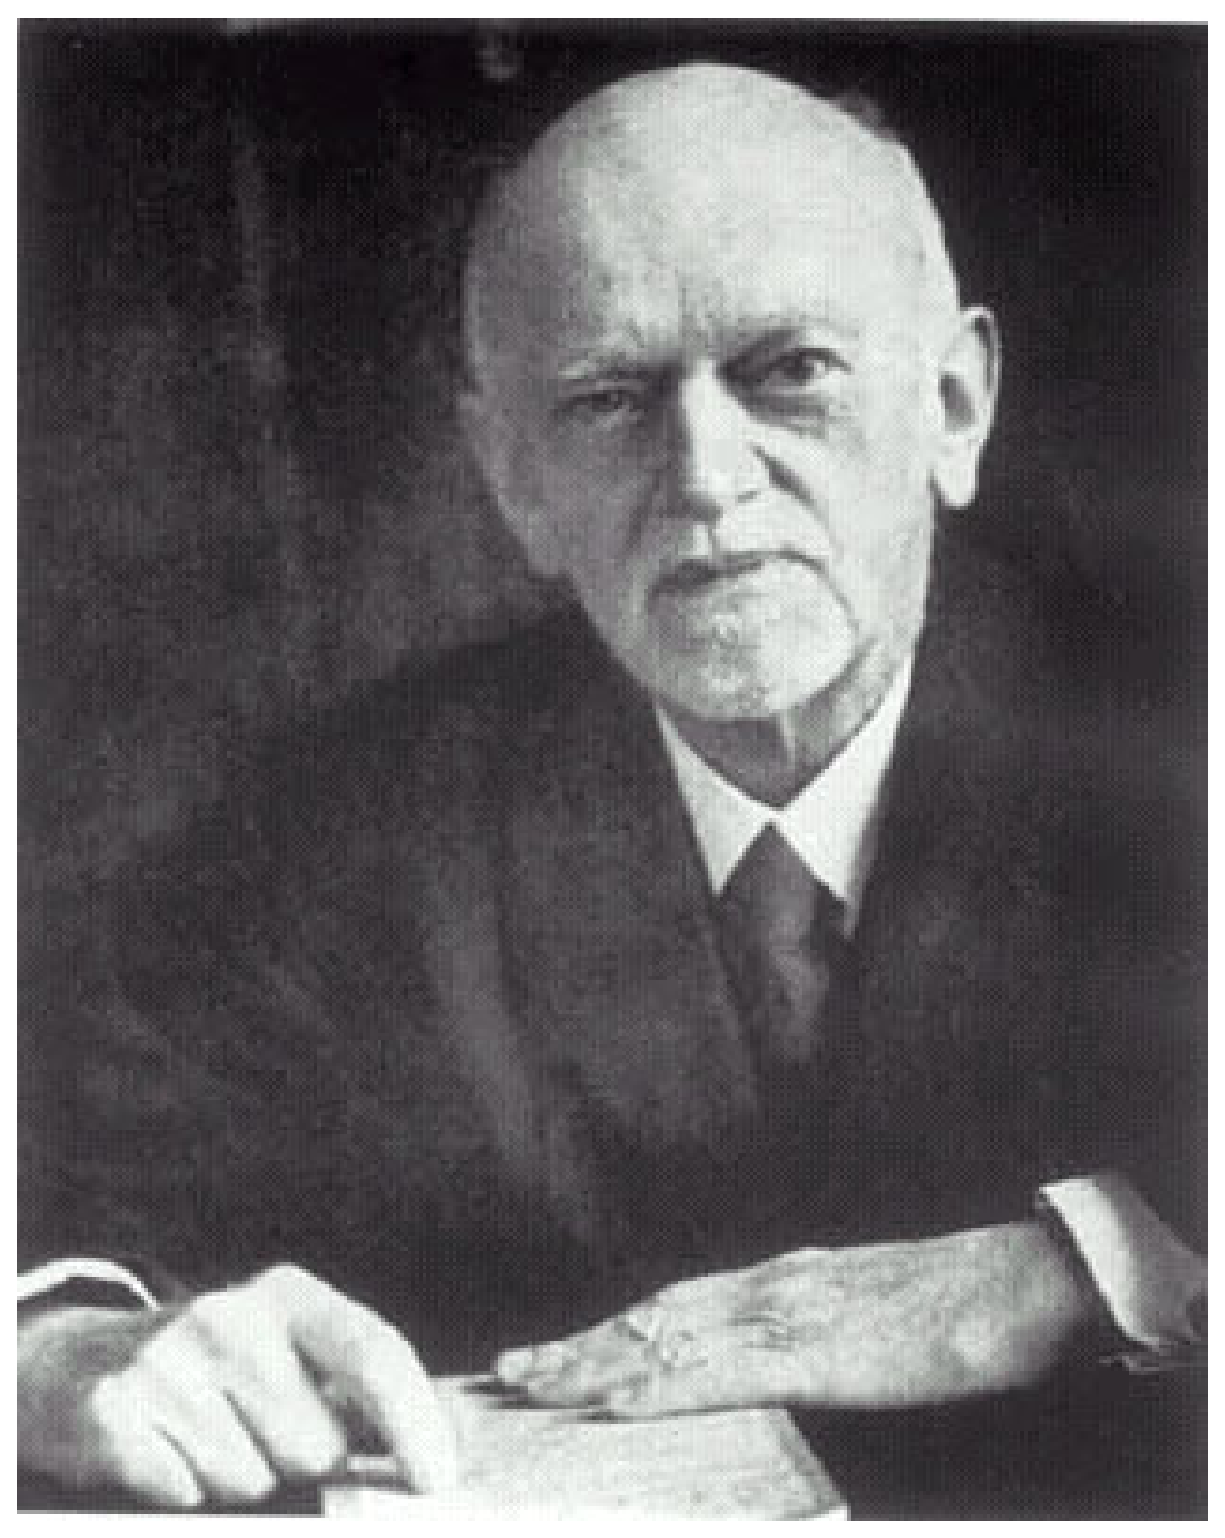
\includegraphics[clip,width=6cm]{WaveFunction/hilbert.ps}
\caption{希尔伯特}
\end{center}
\end{figure}

\subsection{态迭加原理}

如果$\psi _1 ,\psi _2 $是系统两个可能的状态\footnote{根据统计解释,$\left| {c_1 \psi _1 } \right|^2 ,\left| {c_2 \psi _2 } \right|^2 $
分别对应系统处在1,2两个状态的几率。},那么它们的线性迭加:$\psi  = c_1 \psi _1  + c_2 \psi _2 $
也是系统的一个可能状态。

用几率波概念和态迭加原理说明电子双缝干涉实验\footnote{参考第5节 粒子的波动性}:

\index{Double-slit experiment: 双缝实验}

\begin{enumerate}
    \item 双缝,电子出现几率正比于:
    
\begin{eqnarray*}
\left| \psi  \right|^2 &=& \left| {\psi _1  + \psi _2 } \right|^2  = \left( {\psi _1 ^*  + \psi _2 ^* } \right)\left( {\psi _1  + \psi _2 } \right) \\
{} &=& \left| {\psi _1 } \right|^2  + \left| {\psi _2 } \right|^2  + \psi _1 \psi _2 ^*   + \psi _1 ^* \psi _2
\end{eqnarray*}

公式中后两项:

\begin{eqnarray*}
\psi _1 \psi _2 ^*   + \psi _1 ^* \psi _2 &=& \left| \psi_1 \psi_2 \right| \left( e^{i (\theta_1 - \theta_2)} + e^{ - i (\theta_1 - \theta_2)} \right) \\
{} &=& 2 \left| \psi_1 \psi_2 \right| \cos (\theta_1 - \theta_2) 
\end{eqnarray*}

是干涉项,是产生干涉条纹的原因。


    \item 挡住一条缝,或在一条缝处观察到电子穿过,都是等效的,
即都对应一个``纯粹''的态(比如说是态1)。已经在缝1处观察到电子,
意味着电子处在缝1的几率是1,是确定的事件,2态的系数必为零。
所以无干涉条纹产生。
   \end{enumerate}


态迭加原理一般可写为:

\begin{equation}
\psi  = c_1 \psi _1  + c_2 \psi _2  + ... + c_n \psi _n  + ... = \sum\limits_n {c_n \psi _n } 
\end{equation}

当$\left\{ {\psi _i } \right\}$是系统可能状态时,则其线性迭加也是系统可能状态。或说:当系统处于$\psi$时,则$\psi$ 是各可能状态$\left\{ {\psi _i } \right\}$之和。

这其实就是个如何分类的问题,$\left\{ {\psi _i } \right\}$中蕴含着分类的标准。好的分类应该满足两个条件:首先不能遗漏,其次不能重复。比如对三维空间中的向量,笛卡尔坐标系就提供了一个好的分类标准,即一个向量总可以分成延$\hat x$轴的成分,延$\hat y$轴的成分和延$\hat z$轴的成分,它们互相都不包含对方,同时又不遗漏任何成分。当然好的分类标准不只一个,对具体物理问题,我们应选使问题最简化的方案。就刚才的例子而言,除了笛卡尔坐标,我们还有球坐标,还有柱坐标,它们分别适用于不同的物理问题。

量子力学中态所具有的性质与希尔伯特空间中矢量所具有性质是一致的,
因此用希尔伯特空间中矢量可表示量子力学的态。量子力学的数学基础是泛函分析。

根据态迭加原理,电子波函数可表示为具有确定动量波函数:$\psi _p (r,t) = Ae^{\frac{i}{\hbar }(p \cdot r - Et)} $的迭加(即我们按动量$p$给波函数分类)。

首先我们求出归一化因子A:

\begin{eqnarray*}
\int_{ - \infty }^\infty  \psi _p ^* \psi _{p'} d\tau &=& A^2 \int_{ - \infty }^\infty  {\exp \left[ { - \frac{i}{\hbar }\left( {p - p'} \right) \cdot r} \right]}  d\tau  \\
{} &=& A^2 \mathop {\lim }\limits_{N \to \infty } \int_{ - N}^N {\exp \left[ { - \frac{i}{\hbar }\left( {p - p'} \right) \cdot r} \right]} d\tau \\
{} &=& A^2 \mathop {\lim }\limits_{N \to \infty } \frac{{2\sin \left[ {{\textstyle{{(p_x  - p'_x )N} \over \hbar }}} \right]}}{{{\textstyle{1 \over \hbar }}\left( {p_x  - p'_x } \right)}} \cdot \frac{{2\sin \left[ {{\textstyle{{(p_y  - p'_y )N} \over \hbar }}} \right]}}{{{\textstyle{1 \over \hbar }}\left( {p_y  - p'_y } \right)}} \cdot \frac{{2\sin \left[ {{\textstyle{{(p_z  - p'_z )N} \over \hbar }}} \right]}}{{{\textstyle{1 \over \hbar }}\left( {p_z  - p'_z } \right)}} \\
{} &=&  \delta(p_x  - p'_x) \delta(p_y  - p'_y) \delta(p_z  - p'_z) = \delta (p - p')
\end{eqnarray*}

这里我们利用了:

\begin{equation}
\delta (x) = \frac{1}{\pi }\mathop {\lim }\limits_{N \to \infty } \frac{{\sin (Nx)}}{x}
\end{equation}

和

\begin{equation}
\delta (ax) = \frac{1}{a}\delta (x)
\end{equation}

所以:

\begin{equation*}
A^2 (2\pi \hbar )^3 \delta (p - p') = \delta (p - p')
\end{equation*}

求出归一因子:

\begin{equation}
A = \frac{1}{{\left( {2\pi \hbar } \right)^{3/2} }}
\end{equation}

定义归一化波函数:

\index{Normalized wave function: 归一化波函数}

\begin{center}
\begin{equation}
\psi _p (r) = \frac{1}{{\left( {2\pi \hbar } \right)^{{\textstyle{3
\over 2}}} }}\exp \left[ {{\textstyle{i \over \hbar }}(p \cdot r)}
\right]
\end{equation}
\end{center}

根据迭加原理,$\psi(r,t)$可以表示为不同$\psi_p(r)$的迭加,迭加系数为$c(p,t)$:

\begin{equation}
\psi (r,t) = \int\limits_{ - \infty }^\infty  {c(p,t)\psi _p (r)d^3
p}  = \frac{1}{{\left( {2\pi \hbar } \right)^{{\textstyle{3 \over
2}}} }}\int_{ - \infty }^\infty  {c(p,t)\exp \left[ {{\textstyle{i
\over \hbar }}(p \cdot r)} \right]} d\vec p
\end{equation}

$\left| {c(p,t)} \right|^2 $代表波函数$\psi (r,t)$中所含有平面波$\psi _p (r)$的几率,即粒子动量为$p$的几率。

$c(p,t)$可表示为:

\begin{center}
\begin{equation}
   c(p,t) = \frac{1}{{\left( {2\pi \hbar } \right)^{{\textstyle{3 \over 2}}} }}\int_{ - \infty }^\infty  {\psi (r,t)\exp \left[ { - {\textstyle{i \over \hbar }}(p \cdot r)} \right]} d\tau  = \int\limits_{ - \infty }^\infty  {\psi (r,t)\psi _r (p)d\tau }
\end{equation}
\end{center}

这里$\psi _r (p)$是:

\begin{center}
\begin{equation}
    \psi _r (p) = \frac{1}{{\left( {2\pi \hbar } \right)^{{\textstyle{3 \over 2}}} }}\exp \left[ { - {\textstyle{i \over \hbar }}(p \cdot r)} \right]
\end{equation}
\end{center}

\subsubsection*{讨论:}

$c(p,t),\psi (r,t)$互为傅立叶变换。$c(p,t)$确定后,$\psi (r,t)$就完全确定,反之亦然。所以$c(p,t),\psi (r,t)$
是同一个状态的两种不同描述方式。相当于矢量在希尔伯特空间(Hilbert Space)中两不同正交系下的表示(representation)。如以位置为分类标准的波函数$\psi _r (p)$为正交归一基,对应为坐标表象,其系数$\psi (r,t)$是坐标表象下的波函数,如以动量为分类标准的波函数$\psi _p (r)$
为正交归一基,对应为动量表象,其系数$c(p,t)$是动量表象下的波函数,表象变换的实质是希尔伯特空间中的坐标变换。

容易证明,波函数在不同表象下都是归一的,即希尔伯特空间中向量的长度不随基矢的选择而改变。

\begin{equation}
\int\limits_{ - \infty }^\infty  {\left| {c(p,t)} \right|^2 d\mathord{\buildrel{\lower3pt\hbox{$\scriptscriptstyle\rightharpoonup$}}
\over p} }  = \int\limits_{ - \infty }^\infty  {\left| {\psi (r,t)} \right|^2 d\mathord{\buildrel{\lower3pt\hbox{$\scriptscriptstyle\rightharpoonup$}}
\over r} }  = 1
\end{equation}

\textbf{证明:}

动量表象下,几率:

\begin{equation}
w(p,t) = \left| {c(p,t)} \right|^2 d\mathord{\buildrel{\lower3pt\hbox{$\scriptscriptstyle\rightharpoonup$}}
\over p} 
\end{equation}

这里$d \vec p$表示在三维动量空间中的积分,也常常写为$d^3 p$,但为了草稿纸的简洁,我们也经常把它直接写为$d p$。

\begin{eqnarray*}
\int\limits_{ - \infty }^\infty  d\mathord{\buildrel{\lower3pt\hbox{$\scriptscriptstyle\rightharpoonup$}} \over p}  \left| {c(p,t)} \right|^2   & = & \int\limits_{ - \infty }^\infty   d\mathord{\buildrel{\lower3pt\hbox{$\scriptscriptstyle\rightharpoonup$}}
\over p}  {  c^* (p,t)c(p,t) }   \\
{} & = & \int\limits_{ - \infty }^\infty  {d\mathord{\buildrel{\lower3pt\hbox{$\scriptscriptstyle\rightharpoonup$}}
\over p} d\mathord{\buildrel{\lower3pt\hbox{$\scriptscriptstyle\rightharpoonup$}}
\over r} d\mathord{\buildrel{\lower3pt\hbox{$\scriptscriptstyle\rightharpoonup$}}
\over r'} \psi ^* (r,t)\psi (r',t)\frac{{e^{{\textstyle{i \over \hbar }}p \cdot (r - r')} }}{{\left( {2\pi \hbar } \right)^3 }}}  \\
{} & = & \int\limits_{ - \infty }^\infty  {d\mathord{\buildrel{\lower3pt\hbox{$\scriptscriptstyle\rightharpoonup$}}
\over r} d\mathord{\buildrel{\lower3pt\hbox{$\scriptscriptstyle\rightharpoonup$}}
\over r'} \psi ^* (r,t)\psi (r',t)\delta (r - r')} \\
{} & = & \int\limits_{ - \infty }^\infty  {\psi ^* (r,t)\psi (r,t)d\mathord{\buildrel{\lower3pt\hbox{$\scriptscriptstyle\rightharpoonup$}}
\over r} }  =  1
\end{eqnarray*}

\subsection{量子力学中的平均值}

已知归一化波函数$\psi$:

(1)位置的平均值\footnote{``平均值''(average
value)还是``期望值''(expectation value)? 从措辞的角度很微妙,
如果说是``平均值'', 有多次测量然后取平均的意思,
而``期望值''则无此意思。因此说``期望值''比说``平均值''要更严谨一些,
因为这样就没必要复制一大堆相同的波函数了,
即不需要先引入``系综''(Ensemble)的概念。}:

\begin{equation}
\left\langle r \right\rangle  = \int_V {r\psi ^* (r)\psi (r)d\tau  = \int_V {\psi ^* (r)r\psi (r)d\tau }  = \left\langle \psi  \right|} r\left| \psi  \right\rangle 
\end{equation}

(2)动量的平均值:

\begin{equation}
\left\langle p \right\rangle = \sum\limits_k {\hbar k\left| {C_k } \right|^2 }  = \sum\limits_{k'k} {\hbar kC_{k'} ^* C_k \delta _{k'k} }  = \sum\limits_{k'k} {\hbar kC_{k'} ^* C_k \left\langle {{k'}}
 \mathrel{\left | {\vphantom {{k'} k}}
 \right. \kern-\nulldelimiterspace}
 {k} \right\rangle } 
\end{equation}

利用箱归一化波函数$\psi _k (r)$,

\begin{equation}
\psi _k (r)  = \frac{1}{{\sqrt V }}e^{ik \cdot r}
\end{equation}

$\delta _{k'k}$可表示为:

\begin{equation}
\delta _{k'k} = \left\langle k' | k  \right\rangle = \frac{1}{V} \int dr e^{i(k - k') \cdot r} = \frac{1}{V} \int dr e^{-i k' \cdot r} e^{i k \cdot r} 
\end{equation}

动量的平均值可表示为:

\begin{equation}
\left\langle p \right\rangle = \sum\limits_{k' k} C^*_{k'} C_k \int dr \frac{e^{-i k' \cdot r}}{ \sqrt{V}} \hbar k \frac{e^{i k \cdot r}}{ \sqrt{V}}  = \sum\limits_{k' k} C^*_{k'} C_k \int dr  \psi^*_{k'} (r)  \hbar k \psi_k (r)
\end{equation}

考虑到:

\begin{equation}
\frac{\hbar }{i}\nabla \psi_k(r)  = \frac{\hbar }{i}\nabla \frac{e^{ik \cdot r}}{{\sqrt V }}  = \frac{\hbar }{i}(ik)\frac{ e^{ik \cdot r} }{{\sqrt V }}  = \hbar k\psi _k(r) 
\end{equation}

动量的平均值表示为:

\begin{equation}
\left\langle p \right\rangle = \int dr \left( \sum\limits_{k'} C_{k'} \psi_{k'}(r) \right)^* \frac{\hbar}{i}\nabla \left( \sum\limits_k C_k \psi_k (r) \right) = \int dr \psi^*(r) \frac{\hbar}{i}\nabla \psi(r)
\end{equation}

这里的$dr$就是$d \tau$,即对三维空间的积分。

(3)算符的平均值:

在(1)和(2)中我们分别得到坐标表象中的位置算符:$r$,和动量算符:$\frac{\hbar }{i}\nabla$。

一般而言,力学量$A$的平均值可表示为:

\begin{center}
\begin{equation}\label{mean of A}
   \left\langle A \right\rangle  = \left\langle \psi  \right|\hat A\left| \psi  \right\rangle  = \int {\psi ^* \hat A\psi d\tau }
\end{equation}
\end{center}

现在我们可把位置算符$\hat r$和动量算符$\hat p$分别写为:

\begin{eqnarray}
\hat r & = & r \\
\hat p & = & \frac{\hbar}{i }\nabla
\end{eqnarray}

量子力学中常用的算符还有:动能算符$\hat T$、角动量算符$\hat J$、哈密顿算符$\hat H$,……

\subsection{不确定关系的数学推导}

\index{Uncertainty principle: 不确定原理}

假设微观粒子在原点附近运动,使:$\left\langle x \right\rangle  = 0,\left\langle {p_x } \right\rangle  = 0$


则均方偏差为:$\left\langle {\left( {\Delta x} \right)^2 } \right\rangle  = \left\langle {x^2 } \right\rangle ,\left\langle {\left( {\Delta p_x } \right)^2 } \right\rangle  = \left\langle {p_x ^2 } \right\rangle $

\begin{center}
$\begin{array}{l}
 \left\langle {x^2 } \right\rangle  = \int {\psi ^* x^2 \psi dx}  \\
 \left\langle {p_x ^2 } \right\rangle  = \int {\psi ^* \left( { - \hbar ^2 \frac{{\partial ^2 }}{{\partial x^2 }}} \right)\psi dx}  \\
 \end{array}$
\end{center}

考虑积分:$I(\alpha ) = \int_{ - \infty }^\infty  {\left| {\alpha x\psi (x) + \frac{{d\psi (x)}}{{dx}}} \right|^2 dx}  \ge 0,\alpha  \in Real$

\begin{eqnarray*}
I(\alpha ) & = & \alpha ^2 \int_{ - \infty }^\infty  {x^2 \left| \psi  \right|^2 dx}  + \alpha \int_{ - \infty }^\infty  {x\left( {\psi ^* \frac{{d\psi }}{{dx}} + \frac{{d\psi ^* }}{{dx}}\psi } \right)dx}  \\
{} & {} & + \int_{ - \infty }^\infty  {\frac{{d\psi ^* }}{{dx}}\frac{{d\psi }}{{dx}}dx}  \ge 0
\end{eqnarray*}

定义:

\begin{eqnarray*}
A & = & \int_{ - \infty }^\infty  {x^2 \left| \psi  \right|^2 dx}  = \left\langle {x^2 } \right\rangle \\
B & = & - \int_{ - \infty }^\infty  {x\left( {\psi ^* \frac{{d\psi }}{{dx}} + \frac{{d\psi ^* }}{{dx}}\psi } \right)dx = }  - \int_{ - \infty }^\infty  {x\frac{d}{{dx}}\left( {\psi ^* \psi } \right)dx}  \\ 
{} & = & - \left. {x\psi ^* \psi } \right|_{ - \infty }^\infty   + \int_{ - \infty }^\infty  {\psi ^* \psi dx}  = 1 \\
C & = & \int_{ - \infty }^\infty  {\frac{{d\psi ^* }}{{dx}}\frac{{d\psi }}{{dx}}dx}  = \left. {\psi ^* \frac{{d\psi }}{{dx}}} \right|_{ - \infty }^\infty   - \int_{ - \infty }^\infty  {\psi ^* \frac{{d^2 \psi }}{{dx^2 }}dx} \\
{} &= & \frac{1}{{\hbar ^2 }}\int_{ - \infty }^\infty  {\psi ^* \left( { - \hbar ^2 \frac{{d^2 }}{{dx^2 }}} \right)\psi dx}  = \frac{1}{{\hbar ^2 }}\left\langle {p_x ^2 } \right\rangle 
\end{eqnarray*}

这里利用了无穷远处波函数为$0$的条件:

\begin{eqnarray*}
\left. {x\psi ^* \psi } \right|_{ - \infty }^\infty  & = & 0 \\
\left. {\psi ^* \frac{{d\psi }}{{dx}}} \right|_{ - \infty }^\infty & = & 0
\end{eqnarray*}

$I(\alpha ) = A\alpha ^2  - B\alpha  + C \ge 0$,意味着:

\begin{equation*}
B^2  - 4AC = 1 - \frac{4}{{\hbar ^2 }}\left\langle {x^2 } \right\rangle \left\langle {p_x ^2 } \right\rangle  \le 0
\end{equation*}

所以:

\begin{equation}
\left\langle {x^2 } \right\rangle \left\langle {p_x ^2 } \right\rangle  \ge \frac{{\hbar ^2 }}{4}
\end{equation}

考虑到开始的时候我们曾假设粒子在原点附近运动($\left\langle x \right\rangle = 0$,$\left\langle p_x \right\rangle = 0$),上式可改写为:

\begin{center}
\begin{equation}\label{uncertainty relation-7}
    \left\langle {\left( {\Delta x} \right)^2 } \right\rangle \left\langle {\left( {\Delta p_x } \right)^2 } \right\rangle  \ge \frac{{\hbar ^2 }}{4}
\end{equation}
\end{center}


公式\ref{uncertainty relation-7}, 即不确定关系(uncertainty relation)的严格形式。

\subsection{数学补充:$\delta$函数}

\index{Delta function: $\delta$函数}

$\delta$函数的定义:$\delta (x) = \left\{ \begin{array}{l}
 \infty ,x = 0 \\
 0,x \ne 0 \\
 \end{array} \right.$,并满足:$\int_{ - \varepsilon }^{ + \varepsilon } {\delta (x)dx}  = \int_{ - \infty }^{ + \infty } {\delta (x)dx}  = 1$,$\varepsilon$是任意非零无限小量。$\delta$函数是某种分布按参数取极限的过程,
$\delta$函数不是通常意义的函数,它是广义函数。 $\delta$函数是``质点''、``点电荷''、``单位脉冲''等点模型的数学表示。

\subsubsection{$\delta$函数的表示}

$\delta$函数的构造不是唯一的,只要满足$\delta$函数的定义,就是$\delta$函数。

\textbf{例1}:钟形分布 $\rho _\sigma  (x) = \frac{1}{{\sqrt {2\pi
\sigma } }}\exp \left( { - \frac{{x^2 }}{{2\sigma }}}
\right)$,在参数$\sigma  \to 0$极限下,构成$\delta$函数。

首先证明:满足归一条件

定义:$I = \int_{ - \infty }^\infty  {\frac{1}{{\sqrt {2\pi \sigma } }}} \exp \left( { - \frac{{x^2 }}{{2\sigma }}} \right)dx$,显然:$I = \int_{ - \infty }^\infty  {\frac{1}{{\sqrt {2\pi \sigma } }}} \exp \left( { - \frac{{y^2 }}{{2\sigma }}} \right)dy$

所以:$I^2  = \int {\int {\frac{1}{{2\pi \sigma }}\exp \left( { - \frac{{x^2  + y^2 }}{{2\sigma }}} \right)dxdy} } $

极坐标变换:$x^2  + y^2  = r^2 $,$dxdy = rd\theta dr$,积分限:$r \in \left[ {0,\infty } \right]$,$\theta  \in \left[ {0,2\pi } \right]$

利用变量变换:$t = \frac{{r^2 }}{{2\sigma }}$,得到:

$I^2  = \int {\int {\frac{1}{{2\pi \sigma }}\exp \left( { - \frac{{r^2 }}{{2\sigma }}} \right)rd\theta dr} }  = \int_0^\infty  {\frac{1}{{2\sigma }}} \exp \left( { - \frac{{r^2 }}{{2\sigma }}} \right)dr^2  = \int_0^\infty  {{\mathop{\rm e}\nolimits} ^{ - t} dt}  = 1$

所以:$I = \int_{ - \infty }^\infty  {\frac{1}{{\sqrt {2\pi \sigma } }}} \exp \left( { - \frac{{x^2 }}{{2\sigma }}} \right)dx = 1$,满足归一条件。

当$x=0$时,$\mathop {\lim }\limits_{\sigma  \to 0} \rho _\sigma  (x
= 0) \to \infty $;

当$x \ne 0$,$\mathop {\lim }\limits_{\sigma  \to 0} \rho _\sigma  (x) = \mathop {\lim }\limits_{\sigma  \to 0} \frac{1}{{\sqrt {2\pi \sigma } }}\frac{1}{{\exp \left( {{\raise0.5ex\hbox{$\scriptstyle {x^2 }$}
\kern-0.1em/\kern-0.15em
\lower0.25ex\hbox{$\scriptstyle {2\sigma }$}}} \right)}} \to 0$


满足$\delta$函数全部定义,即:

\begin{center}
\begin{equation}\label{delta function bell distribution}
    \delta (x) = \mathop {\lim }\limits_{\sigma  \to 0} \frac{1}{{\sqrt {2\pi \sigma } }}\exp \left( { - \frac{{x^2 }}{{2\sigma }}} \right)
\end{equation}
\end{center}

如令$\alpha  = 1/2\sigma $,式\ref{delta function bell distribution}可改写为:$\delta (x) = \mathop {\lim }\limits_{\alpha  \to \infty } \sqrt {\frac{\alpha }{\pi }} \exp \left( { - \alpha x^2 } \right)$。


常用$\delta$函数的表示:

\begin{itemize}
    \item $\delta (x) = \mathop {\lim }\limits_{\alpha  \to \infty } \frac{{\sin \alpha x}}{{\pi x}}$

    \item $\delta (x) = \mathop {\lim }\limits_{\alpha  \to \infty } \frac{{\sin ^2 \alpha x}}{{\pi \alpha x^2 }}$

    \item $\delta (x) = \mathop {\lim }\limits_{\varepsilon  \to 0} \frac{1}{{2\varepsilon }}\exp \left( { - \frac{{\left| x \right|}}{\varepsilon }} \right)$

    \item $\delta (x) = \frac{1}{\pi }\mathop {\lim }\limits_{\varepsilon  \to 0} \frac{\varepsilon }{{x^2  + \varepsilon ^2 }}$

    \item $\delta (x) = \frac{1}{{2\pi }}\int_{ - \infty }^\infty  {e^{ikx} dk} $

   \end{itemize}

\textbf{例2}:证明$\delta (x) = \mathop {\lim }\limits_{\alpha  \to \infty } \frac{{\sin \alpha x}}{{\pi x}}$

当$x=0$时,$\mathop {\lim }\limits_{\alpha  \to \infty } \frac{{\sin \alpha x}}{{\pi x}} \to \frac{\alpha }{\pi } \to \infty $

当$x \ne 0$时,$\mathop {\lim }\limits_{\alpha  \to \infty } \frac{{\sin \alpha x}}{{\pi x}}$
极限不存在,曲线正负震荡的周期无限缩短。

如考虑积分:$\int_{x \ne 0} {f(x)\left( {\mathop {\lim }\limits_{\alpha  \to \infty } \frac{{\sin \alpha x}}{{\pi x}}} \right)} dx = 0$,即对任何可测函数$f(x)$,$x \ne 0$积分贡献正好抵消。在这个意义上,满足条件$x \ne 0$,$\delta (x) \to 0$。

最后证明积分归一:

\begin{equation*}
\int_{ - \infty }^\infty  {\frac{{\sin \alpha x}}{{\pi x}}dx}  = \int_{ - \infty }^\infty  {\frac{{\sin \alpha x}}{{\pi \alpha x}}} d(\alpha x) = \frac{1}{\pi }\int_{ - \infty }^\infty  {\frac{{\sin t}}{t}dt} 
\end{equation*}

其中:

\begin{eqnarray*}
\int_{ - \infty }^\infty  {\frac{{\sin t}}{t}dt} & = & 2\int_0^\infty  {\frac{{\sin t}}{t}dt}  = 2\int_0^\infty  {\frac{{e^{it}  - e^{ - it} }}{{2it}}} dt  \\
{} & = & \frac{1}{i}\int_0^\infty  {\frac{{e^{it}  - e^{ - it} }}{t}} dt = \frac{1}{i}\int_{ - \infty }^\infty  {\frac{{e^{it} }}{t}dt} \\
{} &  = & \pi 
\end{eqnarray*}

上式积分最后一步,实轴上有单奇点$t=0$,需要利用留数定理\footnote{参考梁昆淼《数学物理方法》,高等教育出版社}进行计算。

所以:

\begin{equation}
\int_{ - \infty }^\infty  {\frac{{\sin \alpha x}}{{\pi x}}dx}  = 1
\end{equation}


\textbf{例3}:证明$\delta (x) = \frac{1}{\pi }\mathop {\lim }\limits_{\varepsilon  \to 0} \frac{\varepsilon }{{x^2  + \varepsilon ^2 }}$


当$x=0$时,$\mathop {\lim }\limits_{\varepsilon  \to 0} \frac{\varepsilon }{{x^2  + \varepsilon ^2 }} = \mathop {\lim }\limits_{\varepsilon  \to 0} \frac{\varepsilon }{{x^2 }} \to \infty $


当$x \ne 0$时,$\mathop {\lim }\limits_{\varepsilon  \to 0} \frac{\varepsilon }{{x^2  + \varepsilon ^2 }} = 0$

只需证明:$\int_{ - \infty }^\infty  {\frac{a}{{x^2  + a^2 }}dx}  = \pi $

变量代换:$x = a\tan \theta $,$dx = a(\sec \theta )^2 d\theta $,积分限:$\left[ { - {\textstyle{\pi  \over 2}},{\textstyle{\pi  \over 2}}} \right]$

\begin{equation*}
\int_{ - \infty }^\infty  {\frac{a}{{x^2  + a^2 }}dx}  = \int_{ - {\raise0.5ex\hbox{$\scriptstyle \pi $}
\kern-0.1em/\kern-0.15em
\lower0.25ex\hbox{$\scriptstyle 2$}}}^{{\raise0.5ex\hbox{$\scriptstyle \pi $}
\kern-0.1em/\kern-0.15em
\lower0.25ex\hbox{$\scriptstyle 2$}}} {\frac{{a^2 \sec ^2 \theta }}{{a^2 \left( {\tan ^2 \theta  + 1} \right)}}d\theta }  = \int_{ - {\raise0.5ex\hbox{$\scriptstyle \pi $}
\kern-0.1em/\kern-0.15em
\lower0.25ex\hbox{$\scriptstyle 2$}}}^{{\raise0.5ex\hbox{$\scriptstyle \pi $}
\kern-0.1em/\kern-0.15em
\lower0.25ex\hbox{$\scriptstyle 2$}}} {d\theta }  = \pi 
\end{equation*}

\textbf{例4}:柯西主值

\begin{equation}
\frac{1}{{x \pm i\varepsilon }} = \frac{{x \mp i\varepsilon }}{{x^2  + \varepsilon ^2 }} = \frac{x}{{x^2  + \varepsilon ^2 }} \mp \frac{{i\varepsilon }}{{x^2  + \varepsilon ^2 }}
\end{equation}

积分:$\mathop {\lim }\limits_{\varepsilon  \to 0} \int_{ - \infty }^\infty  {\frac{{f(x)}}{{x \pm i\varepsilon }}dx}  = \mathop {\lim }\limits_{\varepsilon  \to 0} \int_{ - \infty }^\infty  {\frac{{f(x)x}}{{x^2  + \varepsilon ^2 }}dx}  \mp i\mathop {\lim }\limits_{\varepsilon  \to 0} \int_{ - \infty }^\infty  {\frac{{f(x)\varepsilon }}{{x^2  + \varepsilon ^2 }}} dx$

第2项:

$i\mathop {\lim }\limits_{\varepsilon  \to 0} \int_{ - \infty }^\infty  {f(x)\frac{\varepsilon }{{x^2  + \varepsilon ^2 }}dx}  = i\mathop {\lim }\limits_{\varepsilon  \to 0} \int_{ - \infty }^\infty  {f(x)\pi \delta (x)} dx = i\pi f(0)$


第1项:

\begin{eqnarray*}
{} & {} & \mathop {\lim }\limits_{\varepsilon  \to 0} \int_{ - \infty }^\infty  {f(x)\frac{x}{{x^2  + \varepsilon ^2 }}dx}  = \\
{} & {} & \mathop {\lim }\limits_{\varepsilon  \to 0} \left( {\int_{ - \infty }^{ - \varepsilon } {f(x)\frac{{dx}}{x}}  + \int_\varepsilon ^\infty  {f(x)\frac{{dx}}{x}}  + \int_{ - \varepsilon }^\varepsilon  {f(0)\frac{x}{{x^2  + \varepsilon ^2 }}dx} } \right)
\end{eqnarray*}



其中:$\mathop {\lim }\limits_{\varepsilon  \to 0} \int_{ - \varepsilon }^\varepsilon  {f(0)\frac{x}{{x^2  + \varepsilon ^2 }}dx}  = 0$

定义柯西主值为:

\begin{equation}
P\int_{ - \infty }^\infty  {\frac{{f(x)}}{x}dx}  = \mathop {\lim }\limits_{\varepsilon  \to 0} \left( {\int_{ - \infty }^{ - \varepsilon } {\frac{{f(x)}}{x}dx}  + \int_\varepsilon ^\infty  {\frac{{f(x)}}{x}dx} } \right)
\end{equation}

积分可写为:$\mathop {\lim }\limits_{\varepsilon  \to 0} \int_{ - \infty }^\infty  {\frac{{f(x)}}{{x \pm i\varepsilon }}dx}  = P\int_{ - \infty }^\infty  {\frac{{f(x)}}{x}dx}  \mp i\pi f(0)$

可概括为:

\begin{center}
\begin{equation}\label{cauchy theorem 7}
    \mathop {\lim }\limits_{\varepsilon  \to 0} \frac{1}{{x \pm i\varepsilon }} = P\frac{1}{x} \mp i\pi \delta (x)
\end{equation}
\end{center}

\subsubsection{$\delta$函数的性质:}

\begin{itemize}
    \item $\delta ( - x) = \delta (x)$

    \item $\delta (\alpha x) = \frac{1}{{\left| \alpha  \right|}}\delta (x)$

    \item $\int_{ - \infty }^\infty  {f(x)\delta (x)dx}  = f(0)$

    \item $\int_{ - \infty }^\infty  {f(x)\delta (x - a)dx}  = f(a)$

    \item 如果$\varphi (x) = 0$的实根$x_k (k = 1,2,3,...)$全是单根,则:$\delta \left[ {\varphi (x)} \right] = \sum\limits_k {\frac{{\delta (x - x_k )}}{{\left| {\varphi '(x_k )} \right|}}} $

   \end{itemize}

\subsubsection{$\delta$函数的构造}

任何一组正交归一完备函数集$\left\{ {\psi _n (x)} \right\}$都可用来构成$\delta$函数:
$\delta (x - x') = \sum\limits_n {\psi _n ^* (x')\psi _n (x)} $

任意波函数$\psi$都可以表示为正交归一完备函数集$\psi _n (x)$的展开\footnote{参考: 曾谨言《量子力学 卷I》第729页}:

$\psi (x) = \sum\limits_n {c_n \psi _n (x)} $, $c_n  = \left\langle {{\psi _n }}
 \mathrel{\left | {\vphantom {{\psi _n } \psi }}
 \right. \kern-\nulldelimiterspace}
 {\psi } \right\rangle  = \int {\psi _n ^* (x')\psi (x')dx'} $

\begin{eqnarray*}
\psi (x) & = & \sum\limits_n {\left\langle {{\psi _n }}
 \mathrel{\left | {\vphantom {{\psi _n } \psi }}
 \right. \kern-\nulldelimiterspace}
 {\psi } \right\rangle \psi _n (x)}  = \sum\limits_n {\left( {\int {\psi _n ^* (x')\psi (x')dx'} } \right)\psi _n (x)} \\
{} & = & \int {\left( {\sum\limits_n {\psi _n ^* (x')\psi _n (x)} } \right)} \psi (x')dx'
\end{eqnarray*}

与$\psi (x) = \int {\delta (x - x')\psi (x')dx'} $比较,$\delta (x - x') = \sum\limits_n {\psi _n ^* (x')\psi _n (x)} $。

以上结论在引入狄拉克记号后将变的很好理解,如果不明白,可以暂时先不管它们。


\subsubsection{围道积分}

\index{Contour integration: 围道积分}

考虑积分:$I = \oint_{l} z^n dz$,其中$n$为整数。

\begin{enumerate}
  \item 如果回路$l$不包围原点,积分为$0$;

  \item 如果回路$l$包围原点,$n=0,1,2,...$,积分为$0$;

  \item 如果回路$l$包围原点,$n=-1$,积分为$2\pi i$;

假设$z=Re^{i \theta}$,回路$l$就是按右手法则旋转的闭合圆周,$dz = i
R e^{i \theta} d \theta$,从相位的角度,$dz$比$z$超前$\pi /2$。

\begin{equation*}
 I=\oint \frac{dz}{z} = \int_{0}^{2 \pi} i d \theta =2 \pi i
\end{equation*}


\item 如果回路$l$包围原点,n=$-2,-3,...$,积分为$0$。


\begin{equation*}
 I=\oint \frac{dz}{z^2} = \int \frac{iRe^{i
\theta}d\theta}{R^2e^{i2\theta}}=\frac{i}{R}\int e^{-i\theta}d\theta
= \frac{i}{R}[\frac{e^{-i \theta}}{-i}]_0^{2 \pi} =0
\end{equation*}


这个结果可导致柯西公式和留数定理\footnote{梁昆淼《数学物理方法》pp35}。

柯西公式(Cauchy formula):

\index{Cauchy formula: 柯西公式}

\begin{equation*}
 f(a) = \frac{1}{2\pi i} \oint_l \frac{f(z)}{z-a}dz
\end{equation*}

留数定理(Residue theorem):

\index{Residue theorem: 留数定理}

\begin{equation*}
 \oint_l f(z)dz = 2 \pi i \rm{Res}f(z_0)
\end{equation*}


\end{enumerate}


\subsection{波函数和物理量的取值}

在物理学中, 波函数(wave function)并不是全新的概念。经典的波动,
如一个绷紧的弦上的波动, 可以用一个$\sin$或$\cos$的函数来表示:
$\psi(x,t) = A sin (kx-\omega t +
\phi_0)$。这里的$\psi(x,t)$是有具体物理含义的,
表示弦上$x$位置,$t$时刻, 弦偏离平衡位置的距离。$A$是振幅,
$k$是波矢, $\omega$是角频率,
$\phi_0$是初相位。波动所具有的能量正比于$A^2$, 而与频率无关。

在经典波动中, 我们认为波函数$\psi(x,t)$是实函数, 并对应具体物理量,
在这里$\psi$是弦偏离平衡位置的距离。但把波函数写成复函数会带来数学上的好处,
即: $\psi(x,t) = e^{i(kx-\omega t +
\phi_0)}$。比如我们计算两个波动的迭加问题:$\psi = Acos (kx - \omega
t + \phi_1) + B cos (kx - \omega t + \phi_2)$,
使用复函数就会比使用实函数要直观得多(例如电路分析中的向量模型)。

使用复函数表示波函数,我们立刻可以讨论对于相干波(coherent
wave),$k$同,$\omega$同,如果$\phi_1 -
\phi_2=\pi$,即反相,则发生相消干涉;如果$\phi_1 - \phi_2 =
0$,即同相,则发生相长干涉。光学中的干涉(interference),衍射(diffraction)现象就是这样被解释的。

在经典电动力学中,光波或电磁波也是被表示成类似$\psi(x,t) =
e^{i(kx-\omega t +
\phi_0)}$形式的,但原则上这也是为了数学计算的方便,我们认为光波或电磁波的波函数仍然对应真实物理量,即电场强度($\vec{E}$)和磁场强度($\vec{B}$)。严格说,
经典波动的波函数是需要取实部的,$\psi  = {\mathop{\rm Re}\nolimits}
Ae^{i(kx - \omega t)} $。

如果说``电子是可以用波函数完备地描述的粒子'',
那么就很容易解释电子的干涉实验了。即电子的运动状况不是被($x$,
$p$)描述的,而是被象$\psi = A e^{i(kx - \omega
t)}$这样的波函数描述的,电子的动量由德布洛意关系$p = h/
\lambda$给出。这意味着:

\begin{enumerate}
  \item 在量子力学中, 波函数本身并不对应任何真实物理量,
但我们通过波函数却可获得全部可能的观测量。

  \item 波函数本身虽然不对应任何真实的物理量,
但波函数绝对值的平方却正比于观测到粒子的概率,
即所谓波函数的统计解释(statistical interpretation of wave
function),或玻恩解释(Born interpretation)。
\end{enumerate}

\index{Statistical interpretation: 统计解释}

\index{Born interpretation: 玻恩解释}

比如$\left| \psi(x)
\right|^2$就正比于在$x$附近找到粒子的几率,因此我们总可以找到一个合适的波函数$\psi(x)$,使$\int
\left| \psi(x) \right|^2 dx =
1$,这样的波函数称为归一化波函数(normalized
wave-function)。为了叙述的方便, 我们一般都研究归一化波函数,
对于归一化波函数而言, 几率密度(probability density), $P(x) =
\left| \psi(x) \right|^2$。


那么如何由波函数得到我们真正关心的物理量呢,
比如粒子的位置$x$和粒子的速度$v$?由波函数的统计解释,
我们立刻可以得到粒子位置的期望值(expectation value): $\left\langle
x \right\rangle  = \int {xP(x)dx} $ ,这里的$P(x) = \left| \psi(x)
\right|^2$。但我们无法预测下次测量时粒子的位置,我们只知道粒子在不同位置的概率分布是$\left|
\psi(x) \right|^2$。


在经典物理学中,速度的定义是这样的: $v =\lim \limits_{t_2 \to t_1}
\frac{x_2 - x_1}{t_2 -t_1}$,即$x-t$曲线中的切线。但在量子力学中,
粒子已经没有轨迹概念了, 经典的速度概念自然就失去了意义。看来,
我们在如何由波函数得到速度这个问题上碰到了困难\footnote{我们可以直接对位置的期望值求时间的偏导,
然后利用薛定谔方程和分部积分求出``速度期望值''的表达式,
从而得到动量期望值和动量算符。参考:D. J. Griffith,
\textbf{Introduction to Quantum Mechanics}, pp15。},
那么动量呢?根据德布罗意的工作,我们知道对于单色平面波$\psi = A e^{i
(kx - \omega t)}$而言,$p$就是$\hbar k = h/ \lambda$。因此,有:


\begin{equation*}
    p \psi =\frac{\hbar}{i} \frac{\partial}{\partial x} \psi
\end{equation*}


我们称这样的方程为本征方程(eigen
equation),使方程成立的$p$称为本征值(eigen
value),对应的解$\psi_p (x,t) = \frac{1}{(2 \pi \hbar)^{3/2}}
e^{i(px -Et)/ \hbar}$(已写成归一化的形式),称为本征函数(eigen
function)。对这样的$\psi_p$测量动量,其取值就是$p$,


\begin{equation*}
    p = \int \psi^*_p(x) \frac{\hbar}{i} \frac{\partial}{\partial x}
\psi_p(x) dx
\end{equation*}



对一个一般的波函数,我们可以先把它分解为很多个单色平面波迭加的形式,即:$\psi
= \sum_p A_p
\psi_p$,对每个$\psi_p$,动量都是$p$,其权重正比于$\left| A_p
\right|^2$。动量的期望值为:

\begin{eqnarray*}
\left\langle p \right\rangle &=& \sum_p \left| A(p) \right|^2 p =
\sum_p A^*(p)A(p) \int \psi^*_p(x) \frac{\hbar}{i}
\frac{\partial}{\partial x} \psi_p (x) dx \\
{} & = & \int \psi^*
\frac{\hbar}{i} \frac{\partial }{\partial x} \psi dx
\end{eqnarray*}


回忆一下位置的期望值:$\left\langle x \right\rangle = \int \psi^* x
\psi dx$。我们发现观测量的期望值都可表示为:$\left\langle O
\right\rangle = \int \psi^* \hat O \psi dx$的形式。这里的$\hat
O$是算符(operator),表示对波函数的一种操作,效果上使一个波函数映射为另一个波函数:$\hat
O \psi = \varphi$。


根据经典力学的哈密顿形式,一个物理系统可以用哈密顿量$H(x,p)$描述,其运动状况可以由($x$,
$p$)描述,动力学问题由运动方程(equation of motion)给出,比如哈密顿方程(Hamilton's equations):


\begin{equation*}
    \left\{ \begin{array}{l}
 \dot x = \frac{{\partial H}}{{\partial p}} \\
 \dot p =  - \frac{{\partial H}}{{\partial x}} \\
 \end{array} \right.
\end{equation*}



现在我们已经得到了动量算符($\hat p = \frac{\hbar}{i}
\frac{\partial}{\partial x}$)、位置算符($\hat x =
x$),以及由波函数求解动量期望值和位置期望值的方法,下面我们该研究波函数应当满足的运动方程了。




\subsection*{阅读与思考}

\begin{itemize}
    \item 阅读梁昆淼《数学物理方法》,第五章:傅里叶变换。

\item $I = \int_{ - \infty }^\infty \exp \left( { - \frac{{x^2 }}{{2\sigma }}} \right) dx$
这样的积分叫高斯积分(Gaussian integral),
这种类型的积分及其变形在计算中经常会碰到, 请阅读: 徐一鸿(A. Zee),
\textbf{Quantum field theory in a nutshell}, pp13.

   \end{itemize}


\subsection*{练习}

对波函数$\psi(x) = C \exp \left( - \frac{x^2}{ 2 a^2} \right)$,(1)求归一化因子$C=?$ (2)进一步求以下物理量的期望值:$\left\langle x \right\rangle = ?$, $\left\langle x^2 \right\rangle = ?$, $\left\langle p \right\rangle = ?$和$\left\langle p^2 \right\rangle = ?$。(3)验证对位置和动量符合海森堡不确定关系。 